\documentclass{ifaPoster}

\usepackage[utf8]{inputenc}
\usepackage[ngerman]{babel}
\usepackage{blindtext}
\usepackage{amsmath} % für multline
\usepackage{subfig} % für subfloat
\usepackage{todonotes}

\ifaAuthor{Meret Feldkemper}
\ifaTitle{Kollaborative Problemlösung in modularen Anlagen mittels persönlicher digitaler Assistenz}
\ifaSupervisorA{Dipl.-Ing. Sebastian Heinze}
%\ifaSupervisorB{Dipl.-Ing. Betreuer B}
%\ifaSupervisorC{Dipl.-Ing. Betreuer C}
\ifaProfessor{Prof. Dr.-Ing. habl. Leon Urbas}
\ifaDayOfSubmission{02.05.2019}
\ifaThesis{Diplomarbeit}
\ifaPhoto{DA_files/Passbild.jpg}
 
\begin{document}

\section{Motivation}
Durch Voranschreiten der Automatisierung in der Prozessführung sind Anlagenbediener vor allem in kritischen Situationen für Entscheidungen verantwortlich \cite{bainbridget_ironies_1983}. Der Mensch trifft seine Entscheidungen anhand von Beobachtungen und Erfahrungen. Im Zuge der entwickelten Modularisierungskonzept wird dies zunehmend schwieriger. Die Flexibilität der modularen Anlagen stellt die Anlagenbediener vor die Herausforderung, Probleme nicht mehr auf Grundlage von umfangreiche Erfahrung lösen zu können \cite{mueller_2018}.

Assistenzsysteme können den Anlagenbediener bei Erkennung von Problemen, deren Zusammenhängen und möglichen Lösungsansätzen unterstützen. Dabei ist der Mensch mit einzubeziehen und seine Kompetenzen zu würdigen.

\section{Analyse}
Tritt ein Problem auf, muss der Nutzer darauf aufmerksam gemacht werden. Wichtig für das Assistenzsystem ist nicht nur die Einordnung, wodurch das Problem ausgelöst wurde, sondern auch wie zeitkritisch und wie komplex das Problem ist. Anhand dieser Merkmale sollte sich die Menge und Art der dargestellten Informationen orientieren. Aktuell erhält der Nutzer mit der Prozessführungsebene Informationen über
\begin{itemize}
\item die aktuelle Verschaltung der Module,
\item das Rezept,
\item die Key Performance Indicator,
\item die Services, deren Zustandsübergänge und deren Parameter
\item und die Fließbilder der Module
\end{itemize}
Sollen nun Lösungen für ein entstandenes Problem gefunden werden, sind vor allem die Ziele eines produzierenden Unternehmens zu berücksichtigen. Diese reichen von der Verfügbarkeit von Mitarbeitern bis zum Aufwand Änderungen an der Anlage vorzunehmen.

\section{Konzept}
Das Assistenzsystem begleitet den Nutzer durch den Problemlöseprozess. Es macht ihn mit Meldungen auf Probleme aufmerksam und gibt die Möglichkeit die Situation einzuschätzen und Randbedingungen zu definieren. Anhand der Bedingungen sucht das Assistenzsystem nach Lösungen, die der Nutzer begutachten kann, um eine Entscheidung zu treffen.

Das Design des Assistenzsystems baut auf einer bereits entwickelten PFE auf \cite{} und passt sich anhand des Problemauslösers an.

Anpassung an Zeitdurck, Bereich, 

\begin{figure}[htbp]
\centering
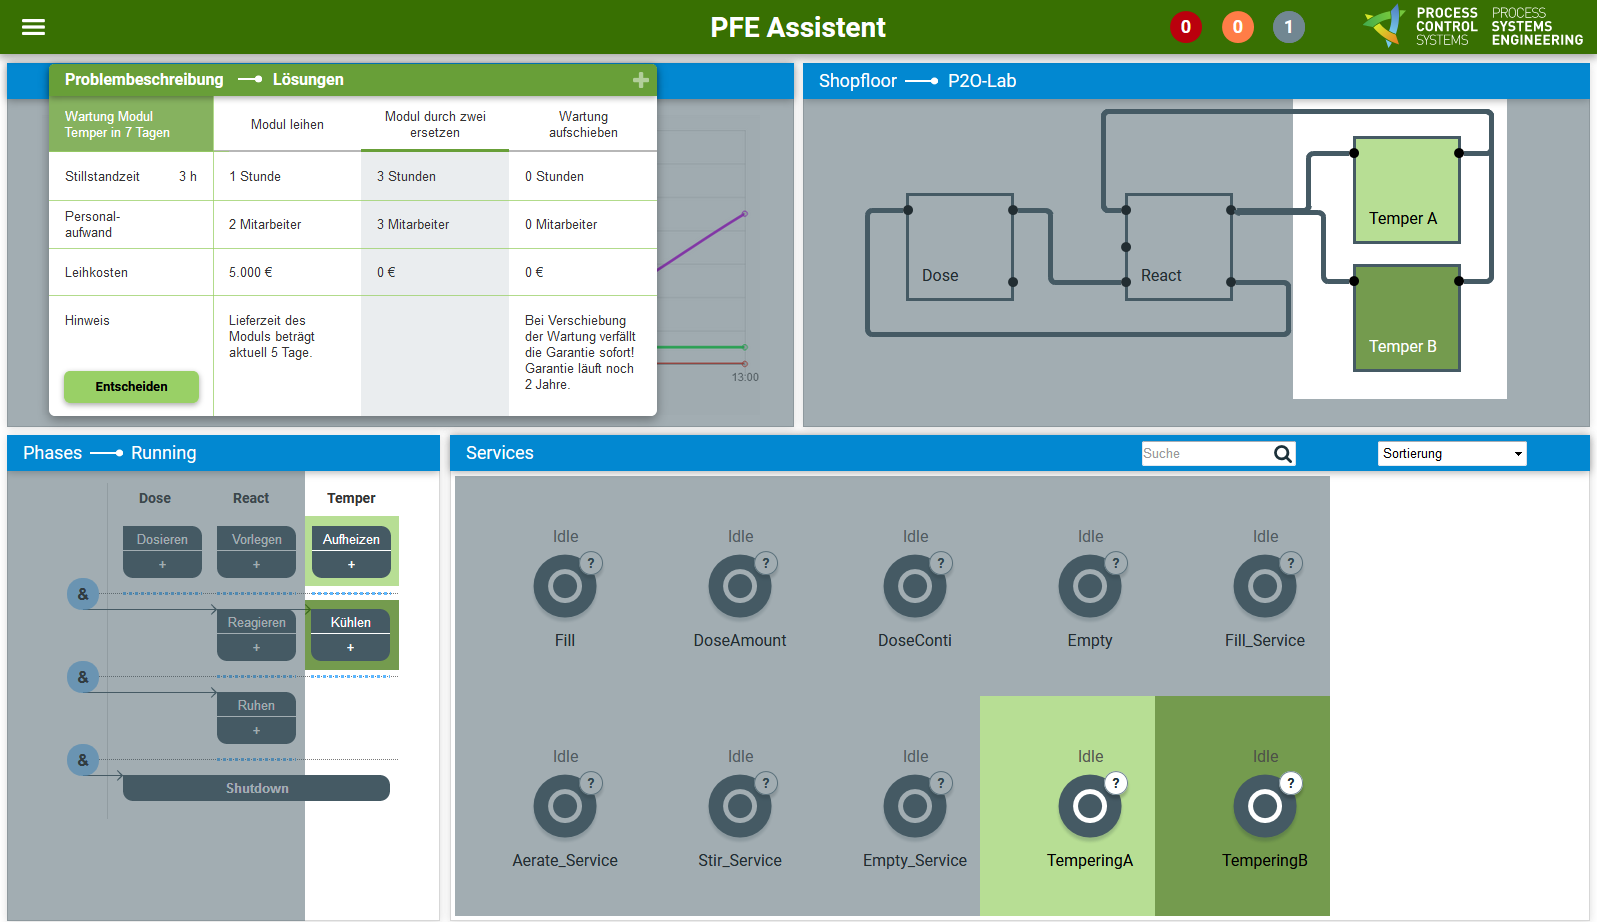
\includegraphics[scale=0.4]{DA_files/Prototyp-PFE-Loesung2.png}
\caption{Darstellung einer Lösung für ein Problem auf Grundlage der PFE}
\end{figure}

\section{Validierung}
Wie gut / schlecht kam der Entwurf an? Was fehlt noch?

Bild vom SUS...



\section{Zusammenfassung und Ausblick}
Nutzer kann mit entsprechenden Informationen geeignet unterstützt werden. Offen bleibt, wie der Nutzer selber Probleme und Lösungen eingeben kann.


 {\tiny\renewcommand{\section}[2]{}%
 	 \begin{thebibliography}{8.5}
 	 \bibitem{bainbridget_ironies_1983}
 	 	Lisanne Bainbridget. {\glqq Ironies of Automation\grqq}. {In: \textit{Automatica}} 19.6 (1983), S. 775-779.
 	 \bibitem{mueller_2018}
 	 Romy Müller. {\glqq Cognitive challenges of changeability: adjustment
to system changes and transfer of knowledge in modular
chemical plants\grqq}. {In: \textit{Cognition, Technology and Work}} 21.1 (2018), S. 113-131.
	\end{thebibliography}}
	
\end{document}